\chapter{Métodos}
En este capítulo se detallan los criterios seguidos para la elección de la geometría de los espaciadores y su escala, los cálculos realizados para la obtención de las propiedades de los materiales utilizados en las simulaciones de transmisión de calor por conducción según la escala utilizada en el modelado 3D del nano-espaciador, los procedimientos seguidos para realizar las simulaciones y el procedimiento seguido para la extracción de los datos de la simulación de CFD.
\section{Criterios de geometría y escala} 
La base del nano-espaciador es cuadrada por ser la más sencilla de fabricar por deposición catódica y para realizar cálculos por ser sus ecuaciones de área y volumen la más sencilla de los polígonos regulares cerrados. El lado de la base del nano-espaciador son de 3$\mu m$ por ser la unidad mínima que se es capaz de depositar en la célula para disminuir las pérdidas por conducción.\\\\
Para el modelado 3D en Inventor se toma como distancia mínima el milímetro, correspondiente a 100nm de la realidad que es la distancia mínima de todos componentes del sistema, para el caso de altura mínima del nano-espaciador a simular.
%%% CALCULOS DE LAS PROPIEDADES DE LOS MATERIALES
\section{Cálculos de las propiedades de los materiales para las simulaciones}
Para obtener los nuevos parámetros de distancias, áreas y volúmenes del modelo 3D del nano-espaciador se procede a obtener las relaciones de escala entre el modelo y la realidad. También se obtienen las relaciones de las propiedades más significativas de los materiales de la realidad y las simulaciones de transmisión de calor por conducción, siendo la principal propiedad la conductividad térmica. Otras propiedades que se toman en cuenta son la densidad y el calor específico, teniendo que destacar la resistencia de contacto por unidad de área entre el nano-espaciador y el emisor.\\\\
Para diferenciar la realidad del modelo 3D o del modelo a simular se utilizará el apostrofe después de la variable correspondiente, por ejemplo, para la longitud real se usa $L$ y para la longitud en el modelo 3D se usa $L'$.\\\\
La relación de longitudes entre el modelo 3D y la realidad es:
\begin{equation}
{L'}/{L}={1mm}/{100nm}=10^4
\label{eq:relacion_longitud}
\end{equation}
%%%  AREA
\subsection{Área}
La sección de los nano-espaciadores es un cuadrado cuya fórmula de área es $A=L^2$, donde $A$ es el área y $L$ el lado del cuadrado, siendo la relación de las áreas la siguiente:
\begin{equation}
	\dfrac{A'}{A}=\left(\dfrac{L'}{L}\right)^2=10^8
	\label{eq:relacion_areas}
\end{equation}
%%% VOLUMEN
\subsection{Volumen}
El volumen de un prisma de base cuadrada se expresa como $V=A\cdot L$, donde $L$ es la altura del prisma.
\begin{equation}
	\dfrac{V'}{V}=\dfrac{A'\cdot L'}{A\cdot L} = 
	\dfrac{A'}{A}\cdot \dfrac{L'}{L} \ \Longrightarrow \ \dfrac{V'}{V} =10^{12}
	\label{eq:relacion_volumen}
\end{equation}
El volumen de cada nano-espaciador en el modelo será $10^{12}$ veces el volumen original.
%%% DENSIDAD
\subsection{Densidad}
La masa de cada elemento es igual entre el modelo($M'$) y la realidad($M$), por lo tanto la densidad varía.
\begin{equation}
\dfrac{\rho '}{\rho}=\dfrac{M'/V'}{M/V}=\dfrac{M'}{M}\cdot \dfrac{V}{V'} \ \Longrightarrow \ 
\dfrac{\rho '}{\rho}=10^{-12}
\label{eq:relacion_densidad}
\end{equation}
La densidad de cada elemento en el modelo será $10^{-12}$ veces la densidad de la realidad.
%%% CONDUCTIVIDAD TERMICA
\subsection{Conductividad Térmica}
La resistencia térmica de los materiales del modelo de simulación se mantiene igual a la de la realidad, por lo tanto, la conductividad térmica de los materiales en el modelo son distintas a la realidad. Sabiendo que la fórmula de la resistencia térmica de conducción es $R=1/k \cdot L/A$, donde $k$ es la conductividad térmica, $L$ la longitud y $A$ es la sección, se puede obtener la relación de las conductividades térmicas del modelo de simulación respecto a la realidad.
\[ \dfrac{R}{R'}= \dfrac{1/k}{1/k'}\cdot \dfrac{L/A}{L'/A'}= \dfrac{k'}{k}\cdot \dfrac{L}{L'}\cdot \dfrac{A'}{A}=1\]
\begin{equation}
\dfrac{k'}{k}=\dfrac{L'}{L}\cdot \dfrac{A}{A'}=\dfrac{10^4}{10^8} \ \Longrightarrow \ \dfrac{k'}{k}=10^{-4}
\label{eq:relacion_conductividadTermica}
\end{equation}
%%% CALOR ESPECIFICO
\subsection{Calor Específico}
El calor específico de los materiales del modelo de simulación es el mismo que el de la realidad porque el calor específico se define como la cantidad de calor necesaria que hay que suministrar a una unidad de masa para elevar su temperatura en una unidad, como la masa del modelo de simulación es igual a la de la realidad, la cantidad de energía necesaria para elevar una unidad de temperatura va a ser igual al del modelo de simulación respecto a la realidad, por lo tanto, el calor específico se mantiene igual al de la realidad.
%%% RESISTENCIA DE CONTACTO
\subsection{Resistencia de contacto}
La resistencia de contacto ($R_c$) es difícil de modelar matemáticamente en una ecuación ya que depende de muchas variables, como la temperatura, presión, entre otros. La resistencia de térmica producida por la resistencia de contacto es $R_{th}=R_{c}/A$, donde A es la superficie de contacto, por lo tanto se ve afectado por la diferencia de escala entre el modelo de simulación y la realidad.
\[ \dfrac{R_{th}'}{R_{th}}=\dfrac{R_c'}{R_c}\cdot \dfrac{A}{A'}=1 \]
\begin{equation}
	\dfrac{R_{th}'}{R_{th}}=\dfrac{R_c'}{R_c}\cdot \dfrac{A}{A'}=1 \ \Longrightarrow \  \dfrac{R_c'}{R_c}=\dfrac{A'}{A}=10^8
	\label{eq:relacion_Rc}
\end{equation}
%%% YOVANOVICH
Para los casos que la resistencia de contacto es presentada como conductancia de contacto según un modelo matemático \cite{experimental_Rc_SS}, según la ecuación de Cooper reducida por Yovanovich (ecuación \ref{eq:modeloYovanovich}).
\begin{subequations}
\begin{equation}
\dfrac{P}{H_c}=\left[ \dfrac{P}{c_1\left(1.62\sigma/m\right)^{c_2}} \right]^{\frac{1}{2+0.071c_2}}
\label{eq:modeloYovanovich}
\end{equation}
\begin{equation}
\dfrac{h_c\sigma}{k_sm}=1.25\left(\dfrac{P}{H_c}\right)^{0.95}
\label{eq:correlacionCooperSimplificadaYovanovich}
\end{equation}
\label{eqs:ecuacionesRcYovanovich}
\end{subequations}
%% Valores de las constantes
Donde $c_1$ es 10.6 GPa, $c_2$ es -0.40, $\sigma$ es la combinación RMS de la rugosidad de ambas superficies de los materiales con $\sigma_i$ siendo la rugosidad de la superficie $i$ (ecuación \ref{eq:mRMS}), $m$ es la combinación RMS de la media absoluta de la pendiente de la rugosidad con $m_i$ siendo la media de la pendiente absoluta de la rugosidad de la superficie $i$ (ecuación \ref{eq:sigmaRMS}), $H_c$ es la micro-dureza Vickers del material más duro y P es la presión aplicada \cite{experimental_Rc_SS}.
\begin{subequations}
\begin{equation}
m=\sqrt{m_1^2+m_2^2}
\label{eq:mRMS}
\end{equation}
\begin{equation}
\sigma=\sqrt{\sigma_1^2+\sigma_2^2}
\label{eq:sigmaRMS}
\end{equation}
\label{eqs:RMS}
\end{subequations}
Las ecuaciones son para la conductancia de contacto ($h_c$) entre dos aceros inoxidables 304(SS304), entonces para tener una mejor idea como la resistencia de contacto afecta a la conducción de calor se supone que el nano-espaciador de $SiO_2$ es liso, por ende, su $m_i$ y su $\sigma_i$ son nulas. Por lo tanto, se calcula la relación de las ecuaciones para el caso de los dos aceros y para el caso de SS-$SiO_2$.\\\\
Como se puede observar en las ecuaciones \ref{eqs:ecuacionesRcYovanovich}, el valor de $\sigma$ y $m$ se presentan siempre relacionados como $\sigma / m$, y se cumple que $\sigma /m =\sigma ' / m'$ porque al suponer que el caso de dos aceros tienen idénticas $m_i$ y $\sigma_i$, la relación $\sigma / m$ queda como $\sigma_i / m_i$, que resulta ser la misma relación para el caso de SS-$SiO_2$.\\\\
\[ \frac{\sigma}{m}=\frac{\sqrt{\sigma_{SS}^2+\sigma_{SS}^2}}{\sqrt{m_{SS}^2+m_{SS}^2}}=\frac{\sigma_{SS}\sqrt{2}}{m_{SS}\sqrt{2}} =\frac{\sigma_{SS}}{m_{SS}}\]
\[ \frac{\sigma'}{m'}=\frac{\sqrt{\sigma_{SS}^2+0^2}}{\sqrt{m_{SS}^2+0^2}}=\frac{\sigma_{SS}}{m_{SS}} \]
Por lo tanto, considerando que $c_1$ y $c_2$ no varían con el cambio de material la relación de $h_c'$ respecto a $h_c$ se obtiene relacionando la ecuación \ref{eq:correlacionCooperSimplificadaYovanovich} del modelo a simular con la realidad.
\[Cte=1.25\frac{m}{\sigma}\cdot \left(\dfrac{P}{H_c}\right)^{0.95} \]
\[h_c=k_s\cdot Cte \qquad k_s=2\cdot \frac{k_1\cdot k_2}{k_1+k_2}\]
Donde $Cte$ es una constante que es igual para el caso de los aceros y el caso SS-$SiO_2$. El valor de $k_s$ para el caso de de los aceros es $k_{SS}$, siendo $k_{SS}$ la conductividad térmica del acero inoxidable 304. 
\[ \frac{h_c'}{h_c}=\frac{k_s'}{k_s}\cdot \frac{Cte}{Cte}=\frac{2 \cdot \frac{k_{SS}\cdot k_{SiO_2}}{k_{SS}+k_{SiO_2}}}{k_{SS}}\]
\begin{equation}
\frac{h_c'}{h_c}=2\cdot \frac{k_{SiO_2}}{k_{SS}+k_{SiO_2}}
\label{eq:relacion_conductividadesTermicas}
\end{equation}
Para este trabajo los datos utilizados de las conductividades térmicas de los materiales para la relación de las conductancias de contacto son a temperatura ambiente, el valor de $k_{SiO_2}$ es $1.5 \ W/\left( m^2 K\right)$ y el valor de $k_{SS}$ es de $15 \ W/\left( m^2 K\right)$, quedando la relación de conductancias de contacto como ${h_c'}/{h_c}=0.1818$.

%%%%%%%%     PROCEDIMIENTOS DE LAS SIMULACIONES Y EXTRACCION DE RESULTADOS
\section{Procedimientos seguidos en la realización de las simulaciones de transmisión de calor y extracción de resultados}
A continuación se describen los procedimientos seguidos en este trabajo para la simulación de la transmisión de calor por radiación de campo cercano, la simulación de la transmisión de calor por conducción y la extracción de los datos de la simulación.\\
\subsection{Para la radiación de campo cercano}
%Aquí tendrías que meter las simulaciones de campo cercano y hablar del método (está descrito en un paper que te pasé
Hay cuatro casos de simulaciones de transmisión de campo cercano que se puede realizar, para este trabajo se realizó una simulación de la combinación de varios materiales con un rango completo de distancias. Para realización de las simulaciones de transmisión de calor por campo cercano de este trabajo, obteniéndose la potencia radiada y la potencia, se siguen los siguientes pasos:
\begin{enumerate}
	\item Abrir la aplicación de la Calculadora de campo cercano.
	\item Seleccionar la cajetilla de \textbf{Materials Range} (figura \ref{fig:check_materials}). 
	\item Seleccionar la cajetilla de \textbf{Distance Range} (figura \ref{fig:check_distances}).
	\begin{figure}[H]%
	\begin{subfigure}[b]{0.48\textwidth}
		\centering
			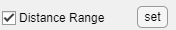
\includegraphics[width=0.6\textwidth]{figuras/Procedimiento_Simulaciones/Radiacion/check_distances2.png}
		\caption{Rango de distancias}
		\label{fig:check_distances}
	\end{subfigure}
	\hfill
	\begin{subfigure}[b]{0.48\textwidth}
		\centering
			
\includegraphics[width=0.6\textwidth]{figuras/Procedimiento_Simulaciones/Radiacion/check_materials2.png}
		\caption{Rango de materiales}
		\label{fig:check_materials}
	\end{subfigure}
	\caption{(\subref{fig:check_distances}) Cajetilla para la selección de la opción de simular un rango de distancias. (\subref{fig:check_materials}) Cajetilla para la selección de la opción de simular una combinación de materiales.}%
	\label{fig:checkboxes}%
	\end{figure}
	\item Hacer clic en el \textbf{set} de \textbf{Materials Range}.
	\item Seleccionar los materiales para el emisor (UpFace) y la célula (DownFace), y hacer clic en aceptar (figura \ref{fig:set_materials}).
	\item Hacer clic en el \textbf{set} de \textbf{Distance Range}.	
	\item Seleccionar el rango de distancias a simular de 100 a 1000 o seleccionar la cajetilla \textbf{Full Range} y hacer clic en aceptar (figura \ref{fig:set_distances}).%% Figuras de las ventanas para los SETs
	\begin{figure}[H]%
	\begin{subfigure}[b]{0.48\textwidth}
		\centering
			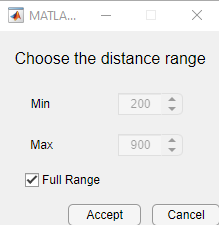
\includegraphics[width=0.6\textwidth]{figuras/Procedimiento_Simulaciones/Radiacion/set_distances_fullrange.png}
		\caption{Set de distancias}
		\label{fig:set_distances}
	\end{subfigure}
	\hfill
	\begin{subfigure}[b]{0.48\textwidth}
		\centering
			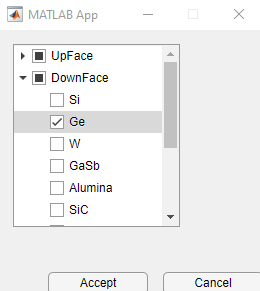
\includegraphics[width=0.6\textwidth]{figuras/Procedimiento_Simulaciones/Radiacion/set_materilas2.png}
		\caption{Set de materiales}
		\label{fig:set_materials}
	\end{subfigure}
	\caption{(\subref{fig:set_distances}) Ventana para la selección del rango de distancias a simular. (\subref{fig:set_materials}) Ventana para la selección de las combinaciones de materiales a simula, siendo \textbf{UpFace} el emisor y \textbf{DownFace} la célula.}%
	\label{fig:sets}%
	\end{figure}
	\item Asegurar que la temperatura del emisor sea la deseada.
	\item Hacer clic en el botón \textbf{Calculate} para lanzar la simulación.
	\item Esperar que el indicador de estado pase de \textit{Running...}, color rojo del indicador (figura \ref{fig:indicador_Running}), a \textit{StdBy}, color verde del indicador (figura \ref{fig:indicador_StdBy}), es decir, esperar que termine la simulación.
	%% figuras de estados
	\begin{figure}[H]
	\centering
	%% Figura 1
	\begin{subfigure}[b]{0.3\textwidth}
	\centering
	
\includegraphics[width=\textwidth]{figuras/Procedimiento_Simulaciones/Radiacion/estado_changed}%
	\caption{Changed}%
	\label{fig:indicador_Changed}%
	\end{subfigure}
	\hfill
	%% Figura 2
	\begin{subfigure}[b]{0.3\textwidth}
	\centering
	
\includegraphics[width=\textwidth]{figuras/Procedimiento_Simulaciones/Radiacion/estado_running}%
	\caption{Running}%
	\label{fig:indicador_Running}%
	\end{subfigure}
	\hfill
	%% Figura 3
	\begin{subfigure}[b]{0.3\textwidth}
	\centering
	
\includegraphics[width=0.9\textwidth]{figuras/Procedimiento_Simulaciones/Radiacion/estado_stdby}%
	\caption{StdBy}%
	\label{fig:indicador_StdBy}%
	\end{subfigure}
	\hfill
	\caption{Indicadores del estado actual del sistema. (\subref{fig:indicador_Changed}) Indicador del estado \textbf{Changed} o estado de cambio, se activa cuando se produce algún cambio en los datos seleccionados para simular. (\subref{fig:indicador_Running}) Indicador del estado \textbf{Running} o corriendo, se activa cuando estando en el estado \textbf{Changed} se hace clic al botón \textbf{Calculate} y corre la simulación. (\subref{fig:indicador_StdBy}) Indicador del estado \textbf{StdBy}, se activa cuando termina la simulación, avisando que está a la espera de algún cambio.}
	\label{fig:indicadorLED}
	\end{figure}
	%% Se acaba la figura
	\item Ir a la pestaña de \textbf{Potencia}.
	\item Introducir el rango de longitudes de onda para calcular la potencia por unidad de área, siendo elegido desde el mínimo hasta 1.8 $\mu m$ que es el rango de longitudes de onda que absorbe la célula de Ge (figura \ref{fig:graficar_ejemplo2}).
	\item Hacer clic en el botón \textbf{Graph} para calcular y graficar las potencias (figura \ref{fig:graficar_ejemplo2}).
\end{enumerate}
%% Graficas de la pestaña de potencia
\begin{figure}[H]
	\centering
	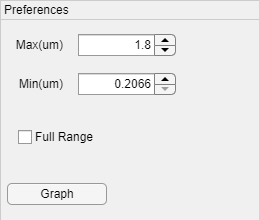
\includegraphics[width=0.30\textwidth]{figuras/Procedimiento_Simulaciones/Radiacion/graficar_ejemplo2.png}
	\caption{Preferencias para el cálculo de la potencia}
	\label{fig:graficar_ejemplo2}
\end{figure}
%% Guardar resultados
El procedimiento seguido en este trabajo se encuentra detallado paos a paso en el Apéndice xxxx. Para la extracción de los datos obtenidos de potencia por unidad de área se hace clic sobre el botón de \textbf{guardar} (figura \ref{fig:SaveButton_Cut}) estando en la pestaña \textbf{Potencia}, para guardar la potencia radiada se hace clic del botón de \textbf{guardar} estando en la pestaña de \textbf{Potencia Radiada} y para guardar todos los datos se hace clic sobre el botón de \textbf{guardar todos} (figura \ref{fig:SaveAllicon}).
\begin{figure}[H]
	\centering
	\begin{subfigure}[b]{0.48\textwidth}
		\centering
		
\includegraphics[width=0.4\textwidth]{figuras/Procedimiento_Simulaciones/Radiacion/SaveButton_Cut.jpg}
		\caption{Botón de guardar actual}
		\label{fig:SaveButton_Cut}
	\end{subfigure}
  \hfill
	\begin{subfigure}[b]{0.48\textwidth}
		\centering
			
\includegraphics[width=0.40\textwidth]{figuras/Procedimiento_Simulaciones/Radiacion/SaveAllicon.jpg}
		\caption{Botón de guardar todos los resultados}
		\label{fig:SaveAllicon}
	\end{subfigure}
	\caption{(\subref{fig:SaveButton_Cut}) Botón de guardar los resultados obtenidos de los cálculos o la simulación, dependiendo de la pestaña que se encuentre el usuario de la calculadora de campo cercano. (\subref{fig:SaveAllicon}) Botón de guardar todos los resultados obtenidos de los cálculos y simulación.}
	\label{fig:saveButtons}
\end{figure}
%%%%%%%%%%%%     Conducción térmica
\subsection{Para la conducción térmica}
Las simulaciones de transmisión de calor por conducción se realizaron todas en CFD, siguiendo un mismo conjunto de pasos. Dichos pasos son los siguientes:
\begin{enumerate}
	\item 
	\item
\end{enumerate}